\documentclass[10pt]{article}
\usepackage[margin=0.9in]{geometry}
\usepackage[T1]{fontenc}
\usepackage{mathptmx}
\usepackage{microtype}
\usepackage{amsmath,amssymb}
\usepackage{graphicx}
\usepackage{booktabs}
\usepackage{tabularx}
\usepackage{array}
\usepackage{xcolor}
\usepackage{caption}
\usepackage[numbers,sort&compress]{natbib}
\usepackage{xr-hyper}
\usepackage[colorlinks=true,linkcolor=blue!50!black,citecolor=blue!50!black,urlcolor=blue!50!black]{hyperref}
\externaldocument{supplement}
\captionsetup{font=small,labelfont=bf}
\setlength{\tabcolsep}{4pt}
\newcommand{\good}[1]{\textcolor{green!45!black}{\textbf{#1}}}
\newcommand{\nsup}[1]{\textcolor{red!60!black}{\textbf{#1}}}
\newcommand{\mixed}[1]{\textcolor{orange!80!black}{\textbf{#1}}}
\renewcommand{\thetable}{\arabic{table}}

\title{\vspace{-1.2em}\textbf{What genome-scale Perturb-seq responses contain: an independent-screen analysis and the limits of reading perturbation responses as regulatory networks}}
\author{Kyler Zook\\\small Department of Electrical Engineering and Computer Science, University of Missouri\\\small\texttt{kylerzook@gmail.com}}
\date{\small Manuscript --- October 2026}

\begin{document}
\maketitle
\vspace{-1em}
\begin{abstract}
\noindent
Perturbation screens are increasingly used both to benchmark expression-prediction models and to infer gene regulatory networks (GRNs). Here, we ask what a CRISPRi knockdown profile in the Replogle 2022 K562 screens actually contains, and how much of it can be interpreted as network structure.

A statistical decomposition of 4{,}507 genome-wide knockdown pseudobulk profiles splits each profile into four parts: a mean (``generic'') direction, a few shared low-rank axes, a residual, and the sampling noise expected from non-targeting controls.
Pooled over knockdowns, expected noise is 47\% of profile energy; for the median knockdown it is 74\% (47--50\% and 74--78\% across noise-constant estimators).
How the remaining signal divides between shared axes and the residual depends strongly on the number of axes removed: the residual is 78\% of signal with none removed, 51\% with three and 18\% with fifty.
When fitted separately in the independent essential-gene screen, the generic direction agrees, and the two three-dimensional shared subspaces share two closely aligned directions, which load on ribosomal and mitochondrially encoded transcripts.

We score held-out predictions against an \emph{independent-screen specific-response target}: the same knockdown measured in the other screen, with the shared structure removed. On this target, the best simple predictor (similarity transfer) reaches a correlation of 0.071 [0.062, 0.080]. That is about 11\% of the ceiling implied by cross-screen agreement under an equal-reliability assumption. On a magnitude-sensitive metric ($R^2$ relative to predicting zero), predictors are near zero or negative on independent-screen targets; after training-only scalar calibration the best specific-target value is 0.004 [0.003, 0.005] (similarity transfer, $k=100$).

A test of whether the knockdown's own responders relay its effect (``cascades'') gives a clear signal on raw and generic-removed profiles. On the specific residual it finds nothing (difference from a random-mediator null $-0.004$ [$-0.012$, $0.004$]). In semi-synthetic positive controls the pipeline detects an injected cascade component carrying 5\% of the signal energy when the mediators are among the knockdown's strongest measured responders, but it loses most or all sensitivity when mediators are ranked arbitrarily or do not respond visibly at the transcript level. The absence of a residual cascade signal is therefore informative only about cascades through strongly responding measured transcripts.

Promoter binding (1~kb upstream, 197 TFs) shows no detectable discrimination of knockdown responders under our responder definition. This holds for measured ChIP-seq binding as well as for motif occupancy, so the failure is not attributable to the occupancy approximation.

Across contexts (Norman 2019; Wessels 2023), strong responses shared by both contexts rarely reverse sign (1.4\% and 1.1\%). Gene-level context differences (nominal $|z_\text{diff}|>3$) occur at 8.5$\times$ and 3.0$\times$ the rate expected under a noise-matched null; reversals are 1.8\% and 1.1\% of these, and the remainder are changes in size, gains, losses and intermediate-strength changes.

Together, these results bound what perturbation responses can say about direct regulatory edges. Simulation studies of model components (memory-based hidden-regulator detection, intervention-induced indirect edges, prior forms, propagation depth) are reported in the Supplement as estimator-specific results.
\end{abstract}

\section{Introduction}
Large Perturb-seq screens \citep{replogle2022} are used for two purposes that are easy to conflate. One is \emph{response prediction}: predicting the transcriptional profile of an unseen perturbation. The other is \emph{network inference}: reading direct regulatory edges out of perturbation responses. Benchmarks have found that sophisticated network-inference methods barely beat simple baselines \citep{chevalley2025causalbench}. Deep response predictors often do not beat linear models or the average perturbation profile \citep{ahlmann2025linear}. Part of this has been traced to systematic variation shared across perturbations, which inflates apparent performance \citep{vinas2026systema}.

Here we characterise what the profiles contain before asking either question. The Replogle K562 data include a genome-wide screen and a separate essential-gene screen, which share 1{,}454 strongly knocked-down targets. Because the screens are independent experiments, sampling noise in one is independent of the other. Comparing them measures reproducible structure (agreement between screens) without a noise model; interpreting the disagreement as noise still requires assumptions. The screens are not exact replicates, however: they were sequenced at different times after transduction (day 8 vs day 6 in the original description \citep{replogle2022}), so disagreement between them also includes biological differences.

\paragraph{Contributions, and how they relate to prior work.}
Systema \citep{vinas2026systema} established that shared perturbation variation inflates apparent predictive performance and proposed evaluating perturbation-specific effects. Our additions are:
(1) a decomposition of genome-scale knockdown responses into expected noise, a generic direction, shared low-rank axes and a residual, with sensitivity analyses and a cross-screen check of both the noise model and the axes;
(2) an \emph{independent-screen} specific-response target with an explicit reliability derivation, used to compare simple predictors on correlation and on a magnitude-sensitive metric;
(3) a cascade (``domino'') test of whether knockdown-specific responses are relayed through the knockdown's measured responders, with a matched positive control;
(4) a promoter-scoped test separating failures of motif occupancy from failures of measured binding to predict knockdown responses;
(5) a noise-matched analysis of context-dependent responses (gained, lost, shared and reversed) in two combinatorial datasets.
Simulation studies of GRN model components, which began this project, are moved to the Supplement and stated as results about the estimators and regimes tested.

\section{Results}

\subsection{A statistical decomposition of knockdown responses}
\label{sec:decomp}
We decomposed 4{,}507 genome-wide knockdown profiles (pseudobulk z-scores; knockdowns with fold expression $<0.5$ and energy-test $p<0.05$; target gene masked). Each profile $x$ is split as
\[x = (x\cdot u)\,u \;+\; V^\top V(x-(x\cdot u)u) \;+\; r,\]
where $u$ is the unit mean knockdown profile (the generic direction), $V$ holds the top $K$ principal axes of the generic-removed matrix, and $r$ is the residual. Expected sampling noise for a profile from $n$ cells is $cG/n$, with $c$ estimated from 585 non-targeting control profiles.
We call the components \emph{generic}, \emph{shared axes} and \emph{specific}. These are statistical labels, not biological ones: shared axes are themselves outputs of regulatory networks, and the residual may contain technical structure.

\paragraph{How much is noise.} Pooled over knockdowns, expected noise is 47\% of total profile energy. The median knockdown is 74\% noise (Table~\ref{tab:decomp}, Fig.~\ref{fig:decomp}a). The pooled figure is lower because a minority of strong knockdowns carries most of the energy. Restricting to the 2{,}000 most variable genes lowers pooled noise to 25\%.
These fractions are stable to the choice of noise-constant estimator (pooled 0.47--0.50, median 0.74--0.78 across profile-level median, mean and trimmed mean and gene-specific estimators) and to resampling of the 585 controls (95\% intervals 0.467--0.473 and 0.733--0.742; Supplementary Table~\ref{tab:s_noise}). These intervals reflect only uncertainty in the noise constant, not misspecification of the noise model.
Allocating expected noise to components in proportion to their dimensionality ($(G-1-K)/G$ to the residual) assumes isotropic noise. Because the shared axes are fitted to the same noisy matrix, they absorb somewhat more than their share of noise, so the specific signal is, if anything, slightly underestimated.

\paragraph{How the signal divides depends on $K$.} The generic share of signal is stable (0.22). The residual's share falls from 0.78 ($K=0$) to 0.51 ($K=3$, the permutation-null choice) and 0.18 ($K=50$) (Fig.~\ref{fig:decomp}b). Shares were broadly similar across tertiles of cell count and knockdown strength; the residual share of signal ranged 0.48--0.61 (Table~\ref{tab:decomp}). Knockdowns with the most cells have the lowest \emph{absolute} expected noise ($cG/n$), but the highest noise \emph{fraction} (median 0.77), because they tend to have weaker responses: knockdowns that impair growth yield fewer cells and stronger effects.

\paragraph{Checks of the noise model and the axes.} We could not split perturbed cells into halves, because only pseudobulk profiles are available. Instead we used the two screens. For a knockdown present in both, $\mathbb{E}\|x_\text{gw}-x_\text{es}\|^2$ equals the sum of both screens' noise energies plus any true between-screen difference.
The observed difference was $1.30\times$ the predicted noise (median ratio; IQR 1.13--1.61). For random pairs of non-targeting profiles the ratio was $1.18\times$ (Table~\ref{tab:noise}). We treat these as consistency checks, not an attribution: they are medians of ratios over different sets of pairs, and the excess can reflect screen or batch effects, extra noise in perturbed profiles, or true between-screen differences. They indicate that the control-calibrated noise model is of the right order but does not account for all cross-screen disagreement.
When the generic direction and three shared axes were fitted separately in each screen, the generic directions agreed ($|\cos|=0.91$). The two three-dimensional subspaces share two closely aligned directions (principal-angle cosines 0.97, 0.94) and not a third (0.01; random subspace 0.02).
Matching individual axes gives the same picture: genome-wide axis 1 matches essential axis 1 ($|\cos|=0.95$) and axis 2 matches axis 2 (0.91), while axis 3 matches nothing (at most 0.12; Supplementary Table~\ref{tab:s_pcmatch}).
The aligned directions load on ribosomal-protein genes and mitochondrially encoded transcripts: aligned direction 1: EEF1A1, TPT1, RPS18, RPS27, SNHG29, RPS3, RPL13A, RPS8; aligned direction 2: MT-CO3, PRG2, MT-ND4, MT-CO2, MT-CO1, MT-ATP6, GAS5, MT-CYB. The non-matching third axis loads on erythroid and haemoglobin genes.
We did not run a formal enrichment analysis, and the mitochondrial direction may be partly technical.

\begin{figure}[t]
\centering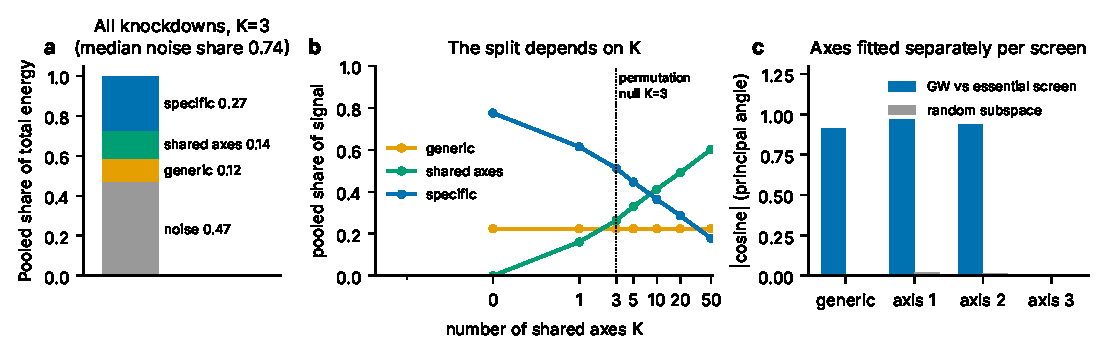
\includegraphics[width=\textwidth]{figures/r1_decomposition.pdf}
\caption{\textbf{Decomposition of 4{,}507 Replogle genome-wide knockdown profiles.} (a) Pooled shares of total energy ($K=3$); the median knockdown's noise share is shown in the title. (b) Pooled shares of signal as a function of the number of shared axes removed. (c) Agreement between generic directions and shared axes fitted separately in the genome-wide and essential-gene screens (1{,}457 knockdowns in both), compared with a random subspace.}
\label{fig:decomp}
\end{figure}

\begin{table}[t]
\centering\small
\caption{\textbf{Decomposition sensitivity.} Pooled quantities are sums over knockdowns divided by total (or signal) energy; ``median noise share'' is the per-knockdown median. ``Specific'' = residual energy minus its expected noise (can be biased by the noise-model error in Table~\ref{tab:noise}).}
\label{tab:decomp}
\resizebox{\textwidth}{!}{\begin{tabular}{lcccc|ccc|c}
\toprule
 & \multicolumn{4}{c|}{Pooled share of total energy} & \multicolumn{3}{c|}{Pooled share of signal} & Median noise \\
Setting & noise & generic & shared axes & specific & generic & shared axes & specific & share / KD \\
\midrule
\multicolumn{9}{l}{\emph{Number of shared axes $K$ (all genes, 4{,}507 knockdowns)}} \\
$K=0$ & 0.47 & 0.12 & 0.00 & 0.41 & 0.22 & 0.00 & 0.78 & 0.74 \\
$K=1$ & 0.47 & 0.12 & 0.09 & 0.33 & 0.22 & 0.16 & 0.62 & 0.74 \\
$K=3$ (permutation null) & 0.47 & 0.12 & 0.14 & 0.27 & 0.22 & 0.26 & 0.51 & 0.74 \\
$K=5$ & 0.47 & 0.12 & 0.18 & 0.24 & 0.22 & 0.33 & 0.45 & 0.74 \\
$K=10$ & 0.47 & 0.12 & 0.22 & 0.19 & 0.22 & 0.41 & 0.36 & 0.74 \\
$K=20$ & 0.47 & 0.12 & 0.26 & 0.15 & 0.22 & 0.49 & 0.29 & 0.74 \\
$K=50$ & 0.47 & 0.12 & 0.32 & 0.09 & 0.22 & 0.60 & 0.18 & 0.74 \\
\midrule\multicolumn{9}{l}{\emph{Gene panel ($K=3$)}} \\
all genes & 0.47 & 0.12 & 0.14 & 0.27 & 0.22 & 0.26 & 0.51 & 0.74 \\
2000 most variable & 0.24 & 0.18 & 0.23 & 0.35 & 0.24 & 0.30 & 0.46 & 0.53 \\
mean UMI $>$ 1 (1728 genes) & 0.30 & 0.14 & 0.26 & 0.30 & 0.21 & 0.37 & 0.43 & 0.57 \\
\midrule\multicolumn{9}{l}{\emph{Cells per knockdown, tertiles ($K=3$; 1 = fewest)}} \\
tertile 1 & 0.46 & 0.13 & 0.15 & 0.26 & 0.24 & 0.28 & 0.48 & 0.67 \\
tertile 2 & 0.48 & 0.11 & 0.13 & 0.29 & 0.21 & 0.24 & 0.55 & 0.77 \\
tertile 3 & 0.53 & 0.08 & 0.11 & 0.29 & 0.17 & 0.23 & 0.60 & 0.77 \\
\midrule\multicolumn{9}{l}{\emph{Knockdown strength, tertiles ($K=3$; 1 = strongest)}} \\
tertile 1 & 0.55 & 0.09 & 0.12 & 0.25 & 0.19 & 0.26 & 0.55 & 0.80 \\
tertile 2 & 0.48 & 0.10 & 0.15 & 0.27 & 0.20 & 0.28 & 0.52 & 0.72 \\
tertile 3 & 0.41 & 0.15 & 0.15 & 0.29 & 0.26 & 0.26 & 0.49 & 0.65 \\
\bottomrule
\end{tabular}}
\end{table}

\begin{table}[t]
\centering\small
\caption{\textbf{Noise-model and axis checks across the two screens.}}
\label{tab:noise}
\begin{tabular}{lc}
\toprule
Check & Value \\
\midrule
Observed / predicted noise energy, gw$-$es difference, same knockdown (1394) & 1.30 [1.13, 1.61] \\
Same, random pairs of non-targeting profiles (300) & 1.18 [0.94, 1.55] \\
$|\cos|$ between generic directions fitted separately per screen & 0.91 \\
Principal-angle cosines, 3 shared axes fitted separately per screen & 0.97, 0.94, 0.01 \\
Same for a random 3-dimensional subspace & 0.02, 0.02, 0.00 \\
\bottomrule
\end{tabular}
\end{table}

\paragraph{The residual reproduces.} For the 1{,}454 knockdowns in both screens, the specific residuals correlate with median $r=0.22$ genome-wide (mismatched knockdowns: $-0.003$). On the 1{,}000 most variable genes used for benchmarking (below) the median is 0.48. Within the genome-wide screen, only 19 targets have a second guide or TSS; their residual agreement was low (median 0.05). Within-screen repeatability therefore cannot be separated from cross-screen agreement in these data.

\subsection{An independent-screen specific-response target}
\label{sec:bench}
\paragraph{Reliability.} Suppose the two screens measure the same underlying response $s$ with independent noise: $x_1=s+e_1$ and $x_2=s+e_2$, with reliabilities $R_i=\operatorname{Var}(s)/\operatorname{Var}(x_i)$. Then
\[\operatorname{corr}(x_1,x_2)=\sqrt{R_1R_2},\qquad \max_f \operatorname{corr}(f,x_2)=\operatorname{corr}(s,x_2)=\sqrt{R_2}.\]
Cross-screen correlation is therefore not itself a ceiling. Under the additional assumption $R_1=R_2$, the best achievable correlation with screen 2 is $\sqrt{r_{12}}$.
If the screens' true responses differ (for example because of timing), $r_{12}$ underestimates the reliability of each screen, and $\sqrt{r_{12}}$ is a conservative (low) estimate of the ceiling for that screen's own response.
Independence removes \emph{shared sampling noise} from the comparison, so a model cannot be rewarded for fitting the same noise realisation it was trained on. It does not remove noise from the target. It also cannot remove dependencies shared by both screens: the same cell line, very probably the same guide designs (guide identities are not in the released pseudobulk files, so we could not verify this), and the same processing pipeline.

\paragraph{Protocol.} Five folds grouped by target gene. Within each fold:
\begin{itemize}
\item The generic direction and shared axes are refitted on training knockdowns only ($K$ by permutation null; 2--4 across folds).
\item The gene panel is the 1{,}000 most variable genes among training knockdowns, chosen per fold.
\item Targets are the held-out knockdown's genome-wide profile, its essential-screen profile (raw, mean-centred by the training mean, and specific residual), with the target gene masked.
\end{itemize}
Similarity transfer predicts a held-out knockdown of gene $t$ as a weighted average of training knockdown profiles. Weights are the correlation between gene $t$'s own expression column and each training target's column, computed across training knockdowns only. This feature uses only training data and is available at prediction time.
The number of neighbours $k\in\{10,20,50,100\}$ was not tuned; all values are reported.
We report Pearson correlation with bootstrap 95\% CIs over held-out knockdowns. As a magnitude-sensitive metric we report $R^2_0=1-\|y-\hat y\|^2/\|y\|^2$ (relative to predicting zero). For constant predictors correlation is undefined and shown as n/a.

\paragraph{Results.} On raw targets the mean training profile scored 0.340 (same screen) and 0.247 (independent screen), close to the best predictor (similarity transfer, $k=100$: 0.374 and 0.285; Table~\ref{tab:bench}, Fig.~\ref{fig:bench}).
Mean-centring the independent-screen target removes the mean profile's credit by construction. Among substantive predictors it gives 0.108--0.135, with the factorised predictor best (0.135 [0.122, 0.148]).
On the specific residual, similarity transfer with $k=100$ was best (0.071 [0.062, 0.080]). Under equal reliability that is about 11\% of the ceiling $\sqrt{r}$ (0.66 on this panel).
Uncalibrated, only the mean profile achieved positive $R^2_0$ on an independent-screen target (raw profiles, 0.007); small-$k$ predictors were strongly negative ($-0.12$ to $-0.19$).
Positive correlation with negative $R^2_0$ can reflect poor amplitude calibration rather than an absence of signal, and averaging over more neighbours shrinks predictions. We therefore calibrated each predictor with a scalar $\hat y_\text{cal}=\lambda\hat y$, with $\lambda\in[0,10]$ chosen on training knockdowns only (leave-one-out predictions for 300 training knockdowns per fold, maximising mean $R^2_0$; $\lambda=0$ allowed).
After calibration (Supplementary Table~\ref{tab:s_f2cal}), all predictors had positive $R^2_0$ on independent raw profiles (0.033 for the mean profile to 0.047 for $k=100$), small positive values on mean-centred targets (0.005--0.013, factorised best) and on specific targets (0.002--0.004; $k=100$: 0.004 [0.003, 0.005]). Fitted factors were below 1 ($\bar\lambda=0.10$--0.46 for similarity predictors), so all predictions were over-scaled.
Paired per-knockdown differences show that more neighbours helps beyond shrinkage on the specific target: $k=100$ minus $k=10$ gives $\Delta$corr $+0.023$ [0.016, 0.030] and, after calibration, $\Delta R^2_0$ $+0.0024$ [0.0016, 0.0031] (Supplementary Table~\ref{tab:s_f2pairs}). $k=100$ and $k=50$ differ little ($\Delta$corr $+0.007$ [0.002, 0.011]; calibrated $\Delta R^2_0$ $+0.0006$ [0.0002, 0.0010]).
The specific target therefore discriminates among substantive predictors, but the explained energy is very small.

\begin{table}[t]
\centering\small
\caption{\textbf{Held-out knockdown prediction} (1{,}396 held-out knockdowns, 5 folds). Correlation with bootstrap 95\% CI; $R^2_0$ = R-squared relative to predicting zero (magnitude-sensitive). n/a: correlation undefined for a constant prediction. Bottom rows: cross-screen agreement of the targets on the same panel and the implied ceiling under equal reliability.}
\label{tab:bench}
\resizebox{\textwidth}{!}{\begin{tabular}{l cc cc cc cc}
\toprule
 & \multicolumn{2}{c}{Same screen, raw} & \multicolumn{2}{c}{Indep., raw} & \multicolumn{2}{c}{Indep., mean-centred} & \multicolumn{2}{c}{Indep., specific} \\
Predictor & corr [95\% CI] & $R^2_0$ & corr [95\% CI] & $R^2_0$ & corr [95\% CI] & $R^2_0$ & corr [95\% CI] & $R^2_0$ \\
\midrule
zero & n/a & -0.000 & n/a & -0.000 & n/a & 0.000 & n/a & -0.000 \\
mean training profile & 0.340 [0.329, 0.350] & 0.042 & 0.247 [0.237, 0.257] & 0.007 & n/a & 0.000 & -0.003 [-0.005, -0.000] & -0.000 \\
kNN k=10 & 0.310 [0.297, 0.322] & -0.189 & 0.244 [0.232, 0.256] & -0.189 & 0.108 [0.094, 0.122] & -0.174 & 0.048 [0.040, 0.056] & -0.120 \\
kNN k=20 & 0.342 [0.330, 0.354] & -0.093 & 0.265 [0.253, 0.277] & -0.117 & 0.116 [0.102, 0.130] & -0.106 & 0.054 [0.046, 0.063] & -0.056 \\
kNN k=50 & 0.369 [0.356, 0.380] & -0.025 & 0.283 [0.271, 0.295] & -0.064 & 0.130 [0.115, 0.144] & -0.056 & 0.064 [0.056, 0.073] & -0.017 \\
kNN k=100 & 0.374 [0.362, 0.386] & 0.003 & 0.285 [0.273, 0.297] & -0.039 & 0.128 [0.114, 0.143] & -0.033 & 0.071 [0.062, 0.080] & -0.004 \\
factorised (generic mean + pathway kNN50 + specific kNN50) & 0.356 [0.343, 0.369] & 0.014 & 0.277 [0.264, 0.289] & -0.017 & 0.135 [0.122, 0.148] & -0.016 & 0.064 [0.056, 0.073] & -0.017 \\
\midrule
Cross-screen $r$ of the target (mean) & -- & -- & \multicolumn{2}{c}{0.59} & \multicolumn{2}{c}{0.58} & \multicolumn{2}{c}{0.47} \\
Ceiling $\sqrt{r}$ (mean; equal reliability) & -- & -- & \multicolumn{2}{c}{0.74} & \multicolumn{2}{c}{0.74} & \multicolumn{2}{c}{0.66} \\
\bottomrule
\end{tabular}}
\end{table}

\begin{figure}[t]
\centering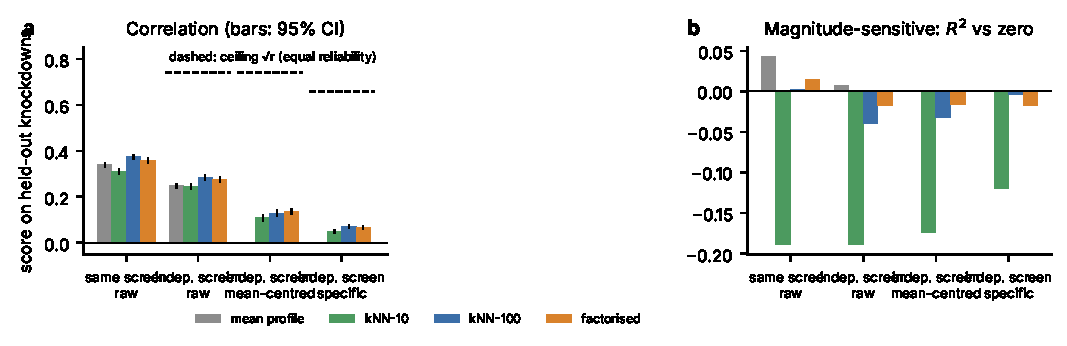
\includegraphics[width=0.95\textwidth]{figures/r2_benchmark.pdf}
\caption{\textbf{Independent-screen evaluation.} (a) Correlation of four predictors with four targets; dashed lines mark the equal-reliability ceiling $\sqrt{r}$ on the same gene panel. (b) $R^2$ relative to predicting zero.}
\label{fig:bench}
\end{figure}

\subsection{Cascade test: is the specific response relayed through the knockdown's own responders?}
\label{sec:domino}
If knockdown $j$ acts largely \emph{through} its strongest responders $k$, its profile should be predicted by $\hat x_j=\sum_k (a_{jk}/d_k)\, x_k$. Here $a_{jk}$ is $j$'s effect on $k$, $d_k$ is $k$'s own knockdown depth, and $x_k$ is $k$'s knockdown profile, which already contains everything downstream of $k$.
We scored $\hat x_j$ against $j$'s profile in the independent screen, excluding $j$ and its mediators from scoring. The null keeps the same weights but uses random mediators.
Mediators are restricted to the 521 genes with a measurable self-knockdown, and we used the 507 targets whose specific residual reproduces across screens (cross-screen $r>0.3$). The estimator sums total effects, so overlapping downstream paths can be counted more than once; it is a linear, one-step reconstruction.

\paragraph{Raw vs residual targets.} The choice of profile determines the result (Table~\ref{tab:domino}, Fig.~\ref{fig:domino}a). On raw profiles, and on profiles with only the generic direction removed, the cascade prediction clearly beats random mediators: difference $+0.137$ [$0.119$, $0.157$] and $+0.133$ [$0.112$, $0.153$]. On the specific residual it does not ($-0.004$ [$-0.012$, $0.004$]).
Cascade-like structure is therefore present, but it lies along the shared axes that residualisation removes. A knockdown's strongest responders have knockdown profiles that resemble its own along those axes. This is consistent with relay through mediators, but equally with co-membership of a complex or pathway; the test cannot distinguish them.

\paragraph{Positive control.} We built semi-synthetic data matched to the real data and ran them through the identical pipeline.
\begin{itemize}
\item For target $j$ with true mediator set $\mathcal{M}_j$ (10 mediators) and weights $w_k$, let $c_j=\sum_{k\in\mathcal{M}_j} w_k r_k$ (real mediator residual shapes $r_k$) and let $o_j$ be $j$'s own real residual shape, orthogonalised against $c_j$. The noise-free target is $s_j=\|r_j\|\,(\sqrt{\alpha}\,\hat c_j+\sqrt{1-\alpha}\,\hat o_j)$, with hats denoting unit vectors. Because $\hat c_j\perp\hat o_j$, $\alpha$ is exactly the fraction of the target's signal energy along the cascade direction; the realised fraction is reported for each run (Supplementary Table~\ref{tab:s_pc2}).
\item Independent Gaussian noise is added for each screen and for each mediator profile, at each profile's real cross-screen reliability.
\item ``Coverage'' hides a fraction of the true mediators from the candidate pool, mimicking mediators that were never knocked down.
\end{itemize}
In the base generator the true mediators are the target's 10 strongest measured responders, the weights are the real $a_{jk}/d_k$, and the target's values at the mediator genes are set to its real effects on them (so the mediators are visible as responders). Under this generator the pipeline detected $\alpha=0.05$ at all coverage levels (Table~\ref{tab:domino_pc}, Fig.~\ref{fig:domino}b), and the real-data upper bound (0.004) lies below the $\alpha=0.05$ lower bound even at 25\% coverage (0.005).
Sensitivity depends strongly on the generator (Supplementary Table~\ref{tab:s_pc2}, Fig.~\ref{fig:domino}c):
\begin{itemize}
\item heterogeneous mediator strengths and halving either screen's reliability reduced but did not remove sensitivity;
\item drawing the true mediators at random among measured genes (ranking errors) reduced sensitivity sharply (at coverage 1: 0.006 at $\alpha=0.05$, 0.023 at $\alpha=0.5$);
\item when the mediators' coordinates in the target were not set to visible responses, the test had no detectable sensitivity even at $\alpha=0.5$;
\item a combination of adverse settings also removed all sensitivity.
\end{itemize}
\textbf{Bounded conclusion:} the pipeline detects a nominal 5\% injected cascade component under the tested semi-synthetic generator, including reduced mediator coverage, provided the mediators are among the knockdown's strongest measured transcript responders. It is not a calibrated exclusion test across plausible generators. In particular, cascades transmitted through mediators whose transcripts respond weakly, or through changes not visible at the transcript level (for example protein activity), are not excluded.
The reliability-normalised share statistic $\max(\mathrm{corr},0)^2/r$ is strongly attenuated by noise (0.11 at $\alpha=1$), so we do not use it as an effect size.

\begin{table}[t]
\centering\small
\caption{\textbf{Cascade test on real data} (507 reproducible knockdowns, 10 mediators; bootstrap 95\% CIs over knockdowns).}
\label{tab:domino}
\begin{tabular}{lcccc}
\toprule
Profiles used (mediators and target) & corr, cascade [95\% CI] & corr, random mediators & difference & frac.\ beats null \\
\midrule
specific residual (original) & -0.010 [-0.015, -0.003] & -0.006 [-0.012, 0.000] & -0.004 [-0.012, 0.004] & 0.47 \\
generic removed only & 0.119 [0.103, 0.136] & -0.014 [-0.024, -0.003] & 0.133 [0.112, 0.153] & 0.71 \\
raw profiles & 0.084 [0.068, 0.100] & -0.054 [-0.068, -0.040] & 0.137 [0.119, 0.157] & 0.75 \\
\bottomrule
\end{tabular}
\end{table}
\begin{table}[t]
\centering\small
\caption{\textbf{Positive control, base generator:} difference between cascade and random-mediator correlations (mean [95\% CI]) for semi-synthetic targets with exact cascade share $\alpha$ (fraction of signal energy) and mediator coverage, run through the same pipeline as Table~\ref{tab:domino}. Robustness to other generators: Supplementary Table~\ref{tab:s_pc2}.}
\label{tab:domino_pc}
\begin{tabular}{lccc}
\toprule
True cascade share $\alpha$ & coverage 1.0 & coverage 0.5 & coverage 0.25 \\
\midrule
0 & 0.000 [-0.003, 0.003] & -0.000 [-0.003, 0.003] & -0.002 [-0.005, 0.001] \\
0.05 & 0.047 [0.044, 0.049] & 0.026 [0.023, 0.029] & 0.008 [0.005, 0.011] \\
0.1 & 0.066 [0.063, 0.069] & 0.038 [0.035, 0.041] & 0.013 [0.010, 0.016] \\
0.25 & 0.106 [0.102, 0.110] & 0.061 [0.057, 0.065] & 0.026 [0.022, 0.030] \\
0.5 & 0.153 [0.147, 0.158] & 0.087 [0.083, 0.092] & 0.039 [0.035, 0.043] \\
\midrule
Real data (specific residual) & \multicolumn{3}{c}{-0.004 [-0.012, 0.004]} \\
\bottomrule
\end{tabular}
\end{table}

\begin{figure}[t]
\centering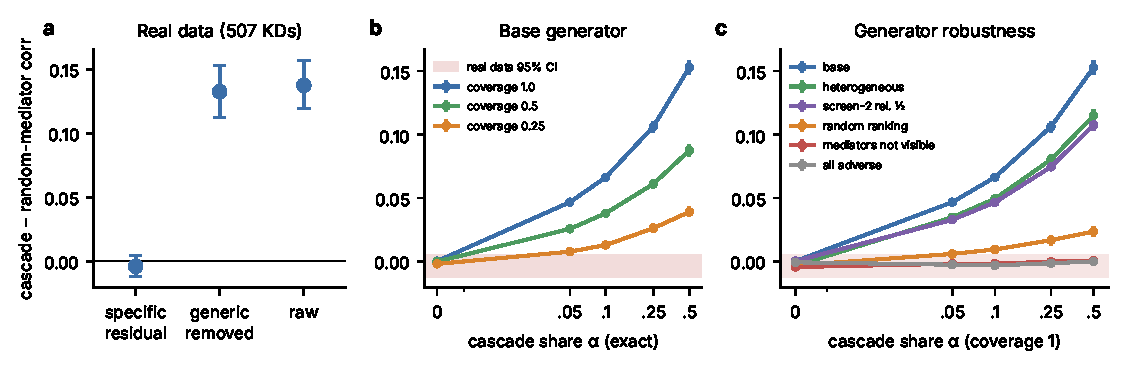
\includegraphics[width=0.92\textwidth]{figures/r3_domino.pdf}
\caption{\textbf{Cascade test.} (a) Real data: cascade prediction minus random-mediator null for three choices of profile. (b) Positive control, base generator: the same statistic for semi-synthetic data with exact cascade share and varying mediator coverage; shaded band = real-data 95\% CI on the specific residual. (c) Sensitivity under alternative generators (coverage 1).}
\label{fig:domino}
\end{figure}

\subsection{Promoter binding does not predict knockdown responders}
\label{sec:binding}
\emph{Scope:} 1-kb upstream promoters of 7{,}839 Perturb-seq-measured genes in K562; ENCODE ChIP-seq (197 TFs); responders defined as genes with $|z|\ge0.5$ in the TF's strongest knockdown (22 TFs with fold expression $<0.85$ and $\ge20$ responders). Distal regulation, TF activity changes and timing are outside this setup.

Motif occupancy weighted by ATAC accessibility predicted ChIP binding better than the maximum motif score (mean per-TF AUROC 0.610 [0.599, 0.621] vs 0.566 [0.555, 0.576]; paired difference 0.045 [0.041, 0.049], higher for 97\% of TFs) and better than accessibility alone (+0.033 [0.022, 0.044]) (Table~\ref{tab:binding}, Fig.~\ref{fig:binding}).
A leave-TF-out ``hub'' score (the fraction of other TFs binding the promoter) predicted binding far better (0.761 [0.753, 0.768]). The hub score correlates moderately with ATAC signal (Spearman 0.33) and expression (0.23), and keeps its AUROC within accessibility or expression quintiles (0.753 and 0.758). Its performance is therefore not fully explained by these coarse stratifications; broadly co-occupied promoters or assay-related structure (for example highly ChIP-able regions) are plausible contributors, but we did not test them directly.

No score predicted knockdown responders: occupancy 0.518 [0.497, 0.542], occupancy$\times$ATAC 0.492 [0.468, 0.520]. Crucially, the same was true of \emph{measured} ChIP binding (0.496 [0.473, 0.511]), including within expression quintiles (0.488).
The failure is therefore not attributable to the occupancy approximation. Measured promoter binding shows no detectable discrimination of responders under this responder definition ($|z|\ge0.5$ in the strongest knockdown); other definitions, distal elements or larger TF sets could behave differently.

\begin{table}[t]
\centering\small
\caption{\textbf{Promoter binding and knockdown response} (per-TF AUROC, bootstrap 95\% CI over TFs).}
\label{tab:binding}
\begin{tabular}{lcc}
\toprule
Score & mean per-TF AUROC [95\% CI] & TFs \\
\midrule
\multicolumn{3}{l}{\emph{Predicting ChIP-seq binding at promoters}} \\
PWM\_max & 0.566 [0.555, 0.576] & 197 \\
occupancy (mu=Ethr-2) & 0.568 [0.557, 0.579] & 197 \\
occupancy x ATAC & 0.610 [0.599, 0.621] & 197 \\
ATAC only & 0.577 [0.569, 0.585] & 197 \\
hub (leave-TF-out binding frequency) & 0.761 [0.753, 0.768] & 197 \\
\midrule \multicolumn{3}{l}{\emph{Within-stratum AUROC (averaged over 5 quintiles)}} \\
hub (leave-TF-out binding frequency) $|$ within ATAC quintile & 0.753 [0.745, 0.761] & 197 \\
occupancy x ATAC $|$ within ATAC quintile & 0.591 [0.581, 0.602] & 197 \\
PWM\_max $|$ within ATAC quintile & 0.566 [0.556, 0.576] & 197 \\
hub (leave-TF-out binding frequency) $|$ within expression quintile & 0.758 [0.750, 0.766] & 197 \\
occupancy x ATAC $|$ within expression quintile & 0.610 [0.599, 0.622] & 197 \\
PWM\_max $|$ within expression quintile & 0.565 [0.555, 0.576] & 197 \\
\midrule \multicolumn{3}{l}{\emph{Predicting knockdown responders ($|z|\ge0.5$)}} \\
ChIP bound (measured binding) & 0.496 [0.473, 0.511] & 22 \\
occupancy (mu=Ethr-2) & 0.518 [0.497, 0.542] & 22 \\
occupancy x ATAC & 0.492 [0.468, 0.520] & 22 \\
PWM\_max & 0.512 [0.493, 0.535] & 22 \\
ChIP bound $|$ within expression quintiles & 0.488 [0.470, 0.502] & 22 \\
occupancy x ATAC $|$ within expression quintiles & 0.494 [0.469, 0.522] & 22 \\
\bottomrule
\end{tabular}
\end{table}

\begin{figure}[t]
\centering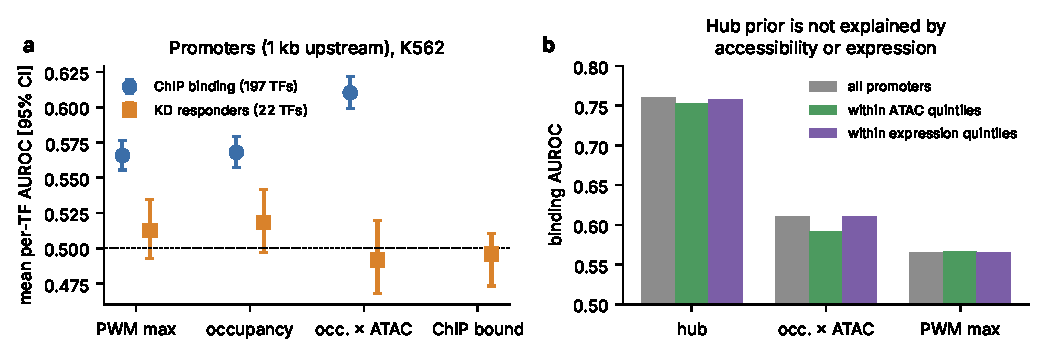
\includegraphics[width=0.92\textwidth]{figures/r4_binding.pdf}
\caption{\textbf{Binding at promoters.} (a) Binding and response prediction by motif, occupancy and measured binding. (b) The hub prior keeps its accuracy within accessibility and expression strata.}
\label{fig:binding}
\end{figure}

\subsection{Context: shared strong responses keep their sign, but many responses change}
\label{sec:context}
We compared the effect of perturbing A alone ($\bar x_A-\bar x_\text{ctrl}$) with its effect in C's context ($\bar x_{AC}-\bar x_C$). This was done for 262 ordered pairs in Norman 2019 \citep{norman2019} (K562, CRISPRa; 2{,}000 variable genes) and 106 in Wessels 2023 \citep{wessels2023} (THP-1, Cas13 knockdown).
These are comparisons of transcriptional \emph{responses}, which combine direct regulation, indirect paths, feedback and state changes. Preserved response signs do not imply preserved signs of direct edges.

Comparing ``significant in one context, not in the other'' is dominated by power: under a null in which both contexts share the same true effect, many genes switch between significant and non-significant by chance. In Wessels, for example, the null predicts more ``lost'' calls than observed (Table~\ref{tab:context}).
We therefore tested each gene directly for a context difference, $z_\text{diff}=(d_2-d_1)/\sqrt{s_1^2+s_2^2}$. The null is matched to each comparison's sampling noise: both contexts share the precision-weighted mean effect, and each estimate is redrawn with its own standard error (20 replicates). $|z_\text{diff}|>3$ is a nominal per-gene threshold without multiple-testing control. We use it to compare aggregate counts with the matched null, which is strong evidence for context dependence overall, not to certify individual genes.

Each significant change is assigned to one category ($z_1$, $z_2$: effect z-scores alone and in context): \emph{reversal}, $|z_1|>3$ and $|z_2|>3$ with opposite signs; \emph{same sign, other size}, both $>3$ with the same sign; \emph{gained}, $|z_1|<1.96$ and $|z_2|>3$; \emph{lost}, $|z_1|>3$ and $|z_2|<1.96$; \emph{other (intermediate strength)}, everything else (at least one effect between 1.96 and 3 in absolute value).

Significant context differences occurred at 8.5$\times$ the null rate in Norman (12{,}084 vs 1{,}421) and 3.0$\times$ in Wessels (1{,}692 vs 562) (Table~\ref{tab:context}, Fig.~\ref{fig:context}).
As a fraction of all significant changes (Norman; Wessels): reversals 1.8\%; 1.1\%; same sign, other size 23.3\%; 4.6\%; gained 26.0\%; 28.7\%; lost 25.3\%; 29.4\%; other (intermediate strength) 23.6\%; 36.3\%.
As a fraction of strong responses shared by both contexts ($|z|>3$ in both), reversals were 1.4\% (218 of 15{,}778) and 1.1\% (18 of 1{,}657).
In Shifrut 2018 \citep{shifrut2018} (T cells, with vs without stimulation), knockout effects were too weak to test: split-half replicates shared only 6--12 strong targets across 18 knockouts (Supplementary Table~\ref{tab:s_f6}).
\textbf{Conclusion:} among strong responses present in both contexts, signs are preserved for $\approx$99\%. However, context-dependent changes in aggregate, including gains and losses of responses, are common and well above noise, so context does not merely rescale a fixed set of responses.

\begin{table}[t]
\centering\small
\caption{\textbf{Context-dependent responses vs a noise-matched null} (counts of gene $\times$ comparison, summed over comparisons; null mean $\pm$ s.d.\ over 20 replicates). The null shares a precision-weighted mean effect across contexts, which makes it generous to ``gained''/``lost'' counts (conservative for claiming context dependence).}
\label{tab:context}
\resizebox{\textwidth}{!}{\begin{tabular}{lrrrr}
\toprule
 & \multicolumn{2}{c}{Norman 2019 (262 comparisons)} & \multicolumn{2}{c}{Wessels 2023 (106 comparisons)} \\
Gene-level category (summed over comparisons) & observed & matched null & observed & matched null \\
\midrule
strong alone ($|z|>3$) & 64,962 & 77,544 $\pm$ 186 & 7,848 & 10,421 $\pm$ 76 \\
strong in context & 26,311 & 28,060 $\pm$ 79 & 5,168 & 7,984 $\pm$ 84 \\
shared, same sign & 15,560 & 20,647 $\pm$ 75 & 1,639 & 2,811 $\pm$ 31 \\
shared, reversed sign & 218 & 3 $\pm$ 2 & 18 & 0 $\pm$ 0 \\
gained (alone $|z|<1.96$) & 7,256 & 4,033 $\pm$ 50 & 2,714 & 3,461 $\pm$ 62 \\
lost (context $|z|<1.96$) & 36,891 & 39,618 $\pm$ 169 & 4,844 & 5,209 $\pm$ 71 \\
significant change, $|z_\mathrm{diff}|>3$ & 12,084 & 1,421 $\pm$ 34 & 1,692 & 565 $\pm$ 23 \\
\quad of which reversal & 218 & 3 $\pm$ 2 & 18 & 0 $\pm$ 0 \\
\quad of which same sign, other size & 2,813 & 50 $\pm$ 8 & 77 & 3 $\pm$ 2 \\
\quad of which gained & 3,136 & 553 $\pm$ 15 & 486 & 162 $\pm$ 10 \\
\quad of which lost & 3,061 & 227 $\pm$ 18 & 497 & 135 $\pm$ 10 \\
\quad of which other (intermediate strength) & 2,856 & 589 & 614 & 264 \\
\bottomrule
\end{tabular}}
\end{table}

\begin{figure}[t]
\centering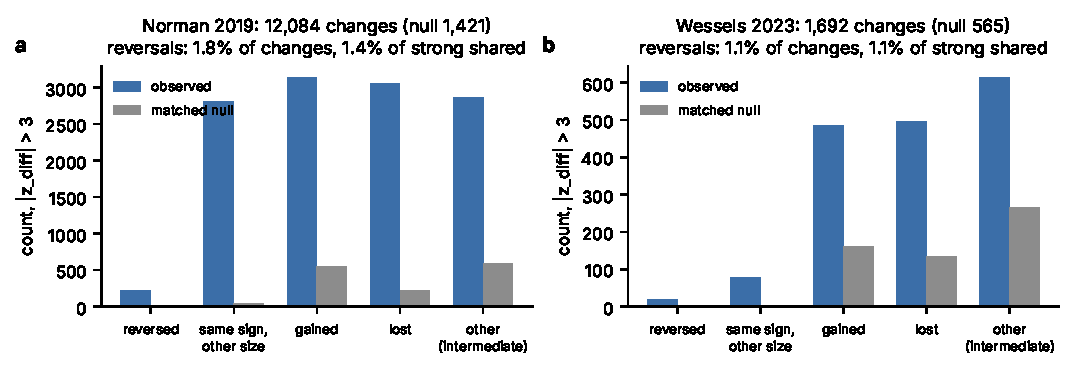
\includegraphics[width=0.92\textwidth]{figures/r5_context.pdf}
\caption{\textbf{Composition of significant context-dependent changes} (nominal $|z_\text{diff}|>3$) in (a) Norman 2019 and (b) Wessels 2023, against a noise-matched null. All five categories are shown; they sum to the total.}
\label{fig:context}
\end{figure}

\section{Discussion}
Three conclusions follow, each with stated limits.

\emph{First}, most of a typical knockdown profile is sampling noise, and much of the signal lies on a generic direction and a few shared axes. Two of these shared directions reproduce across screens and load on ribosomal and mitochondrially encoded transcripts. How much signal is ``specific'' is not a fixed number: it depends on how many shared axes one removes. Benchmarks and network-inference methods should report their choice and its sensitivity.

\emph{Second}, scoring against the independent screen's specific response is a stricter target than raw profiles. It discriminates among substantive predictors, and simple predictors recover only a small fraction of its estimated ceiling. Unlike Systema \citep{vinas2026systema}, which re-scores predictions within a dataset, the independent screen protects against rewarding a model for fitting the same noise realisation. The ceiling derivation makes explicit what cross-screen agreement does and does not bound.

\emph{Third}, perturbation responses are poor direct readouts of regulatory edges in these data. Measured promoter binding does not predict responders. The knockdown-specific residual shows no detectable relay through the knockdown's strongly responding measured transcripts, a test with demonstrated sensitivity only under a favourable generator. Relay-like structure is visible along shared axes, where cascades and shared module membership cannot be told apart. Response-level context dependence is common even though reversals of strong responses are rare.
Models that map perturbation responses to edges therefore need either additional data that resolve direct regulation (for example acute perturbations, time courses, or direct binding-and-response assays), or explicit components for shared response structure.

\paragraph{Limitations.}
\begin{itemize}
\item All Replogle analyses use pseudobulk z-scores. Split-half validation of the noise model on perturbed cells was not possible, and the cross-screen check indicates the noise model is approximate.
\item The two screens differ in timing, and probably share guide designs and processing, so cross-screen agreement mixes noise with biology and may share technical dependencies.
\item The cascade test is linear and one-step. Its sensitivity is demonstrated only under generators in which mediators are visible as strong transcript responders; it is not a calibrated exclusion test.
\item Binding conclusions are limited to proximal promoters in K562.
\item Context analyses compare responses, not edges, and the null uses estimated effects as truth.
\item The simulations in the Supplement concern our own simulator and estimators; the regulator-mask benefit disappears when a quarter of true regulators are missing from the annotation (Supplement S7).
\end{itemize}

\section{Methods}
\paragraph{Replogle data.} K562 genome-wide and essential-gene normalised pseudobulk files (\texttt{K562\_gwps\_normalized\_bulk\_01}, \texttt{K562\_essential\_normalized\_bulk\_01}; \texttt{.h5ad}), Replogle et al.\ 2022 (figshare release accompanying the paper). The gene-level values are the released normalised (z-scored relative to controls) pseudobulk expression changes.
Knockdowns: not non-targeting, fold expression $<0.5$, energy-test $p<0.05$ (4{,}507). The target gene's own column is set to 0.
Essential-screen profiles were mapped to shared genes (8{,}200) and the strongest knockdown per target used.
\paragraph{Decomposition.} The generic direction $u=\bar x/\|\bar x\|$. Shared axes are the top-$K$ right singular vectors of the generic-removed matrix (randomized SVD). The permutation null is the top singular value after shuffling each gene's column independently.
Noise energy is $cG/n$ with $c=\operatorname{median}(\|x\|^2 n/G)$ over non-targeting profiles; the residual's expected noise is scaled by $(G-1-K)/G$.
Pooled shares are sums over knockdowns; medians are per knockdown. Cross-screen axis stability uses principal-angle cosines (singular values of $V_aV_b^\top$).
\paragraph{Benchmark.} As described in Section~\ref{sec:bench}. Bootstrap CIs use 2{,}000 resamples of held-out knockdowns.
\paragraph{Cascade test.} Mediators: knocked-down genes with raw self z $<-1$ (521). Responders: top-$K$ mediators by $|$screen-1 profile at the mediator's column$|$. Weights: $a_{jk}/d_k$, with $a_{jk}$ the raw z of $j$'s knockdown on gene $k$ and $d_k$ the self z of $k$'s knockdown.
Targets with cross-screen residual $r>0.3$ (507). Scoring excludes $j$ and the selected mediators. Null: random mediators with the same weights. Positive control: as in Section~\ref{sec:domino}; noise s.d.\ per profile set so that its expected reliability equals the real cross-screen $r$ (clipped to [0.05, 0.95]).
\paragraph{Binding.} Promoters: 1~kb upstream of refGene TSSs (hg38). Energies: JASPAR 2024 \citep{jaspar2024} PWM log-odds, scanned on both strands. $E_\text{thr}$ is the 10$^{-4}$ quantile of scores on background sequences with promoter base composition; occupancy $=\sum_\text{sites}\sigma(\mu-E)$ at $\mu=E_\text{thr}-2$, and the accessibility-weighted version adds the log ATAC signal at each position.
ChIP: ENCODE K562 conservative IDR peaks \citep{encode2020} (accessions in \texttt{data/raw/encode\_manifest.tsv}). Hub: fraction of the other 196 TFs whose peaks overlap the promoter. Expression: Replogle gene-level mean UMI.
\paragraph{Context.} Norman 2019: log-normalised (CP10k) single-cell matrix, 2{,}000 most dispersed genes, perturbed genes masked. Wessels 2023: scPerturb h5ad \citep{peidli2024scperturb}, same normalisation, perturbations with $\ge60$ cells (singles) and $\ge100$ (pairs). Standard errors are $\sqrt{\operatorname{Var}/n}$ for each group mean.
\paragraph{Uncertainty.} Bootstrap over knockdowns, TFs or targets as stated. Paired comparisons between predictors use per-knockdown differences. Seeds for simulations are listed in the Supplement.
\paragraph{Code and data availability.} Code, results, environment specifications and the commands used are at \url{https://github.com/kylerzook/cross-screen-perturbseq} (release tag \texttt{v1.2}; \texttt{README.md}, \texttt{run\_all.sh}). The main-text pipeline (decomposition, noise and axis checks, binding from cached promoter features, Norman preprocessing and context analysis, benchmark and cascade test) was re-run from a fresh clone in a clean environment built from \texttt{requirements.txt}; all re-computed values matched the reported results exactly, except Monte Carlo null replicates in the context analysis, whose comparison order depended on Python's hash seed; the order is now fixed and the output verified to be deterministic. Commands for the Supplement simulations are supplied as used but were not re-verified end to end. An archived release with a DOI will be added on acceptance. Data identifiers are listed in \texttt{data/README.md}: the Replogle figshare files; ENCODE accessions; JASPAR 2024 CORE vertebrates non-redundant; MotifCentral v1.0.0 (ProBound); scPerturb h5ad files for Wessels and Shifrut; Norman 2019 (GEO GSE133344).

\begin{thebibliography}{99}\small
\bibitem{replogle2022} J.~M.~Replogle et al. Mapping information-rich genotype--phenotype landscapes with genome-scale Perturb-seq. \emph{Cell} 185, 2559--2575 (2022).
\bibitem{chevalley2025causalbench} M.~Chevalley, Y.~Roohani, A.~Mehrjou, J.~Leskovec, P.~Schwab. A large-scale benchmark for network inference from single-cell perturbation data. \emph{Communications Biology} 8, 412 (2025).
\bibitem{ahlmann2025linear} C.~Ahlmann-Eltze, W.~Huber, S.~Anders. Deep-learning-based gene perturbation effect prediction does not yet outperform simple linear baselines. \emph{Nature Methods} (2025).
\bibitem{vinas2026systema} R.~Vi\~nas~Torn\'e et al. Systema: a framework for evaluating genetic perturbation response prediction beyond systematic variation. \emph{Nature Biotechnology} 44, 1050--1059 (2026).
\bibitem{norman2019} T.~M.~Norman et al. Exploring genetic interaction manifolds constructed from rich single-cell phenotypes. \emph{Science} 365, 786--793 (2019).
\bibitem{wessels2023} H.-H.~Wessels et al. Efficient combinatorial targeting of RNA transcripts in single cells with Cas13 RNA Perturb-seq. \emph{Nature Methods} 20, 86--94 (2023).
\bibitem{shifrut2018} E.~Shifrut et al. Genome-wide CRISPR screens in primary human T cells reveal key regulators of immune function. \emph{Cell} 175, 1958--1971 (2018).
\bibitem{jaspar2024} I.~Rauluseviciute et al. JASPAR 2024: 20th anniversary of the open-access database of transcription factor binding profiles. \emph{Nucleic Acids Res.} 52, D174--D182 (2024).
\bibitem{encode2020} ENCODE Project Consortium. Expanded encyclopaedias of DNA elements in the human and mouse genomes. \emph{Nature} 583, 699--710 (2020).
\bibitem{peidli2024scperturb} S.~Peidli et al. scPerturb: harmonized single-cell perturbation data. \emph{Nature Methods} 21, 531--540 (2024).
\end{thebibliography}

\end{document}
